\documentclass[tikz,border=6pt]{standalone}
\usepackage{tikz}
\usetikzlibrary{arrows.meta, positioning, fit, backgrounds, calc}
\usepackage[T1]{fontenc}
\usepackage{helvet}
\usepackage{amsmath,amssymb}
\renewcommand{\familydefault}{\sfdefault}

\definecolor{cData}{HTML}{E3F2FD}
\definecolor{cDataB}{HTML}{1565C0}
\definecolor{cTrain}{HTML}{E8F5E9}
\definecolor{cTrainB}{HTML}{2E7D32}
\definecolor{cVal}{HTML}{FFF3E0}
\definecolor{cValB}{HTML}{E65100}
\definecolor{cOut}{HTML}{ECEFF1}
\definecolor{cOutB}{HTML}{37474F}
\definecolor{cXAI}{HTML}{F3E5F5}
\definecolor{cXAIB}{HTML}{6A1B9A}

\begin{document}
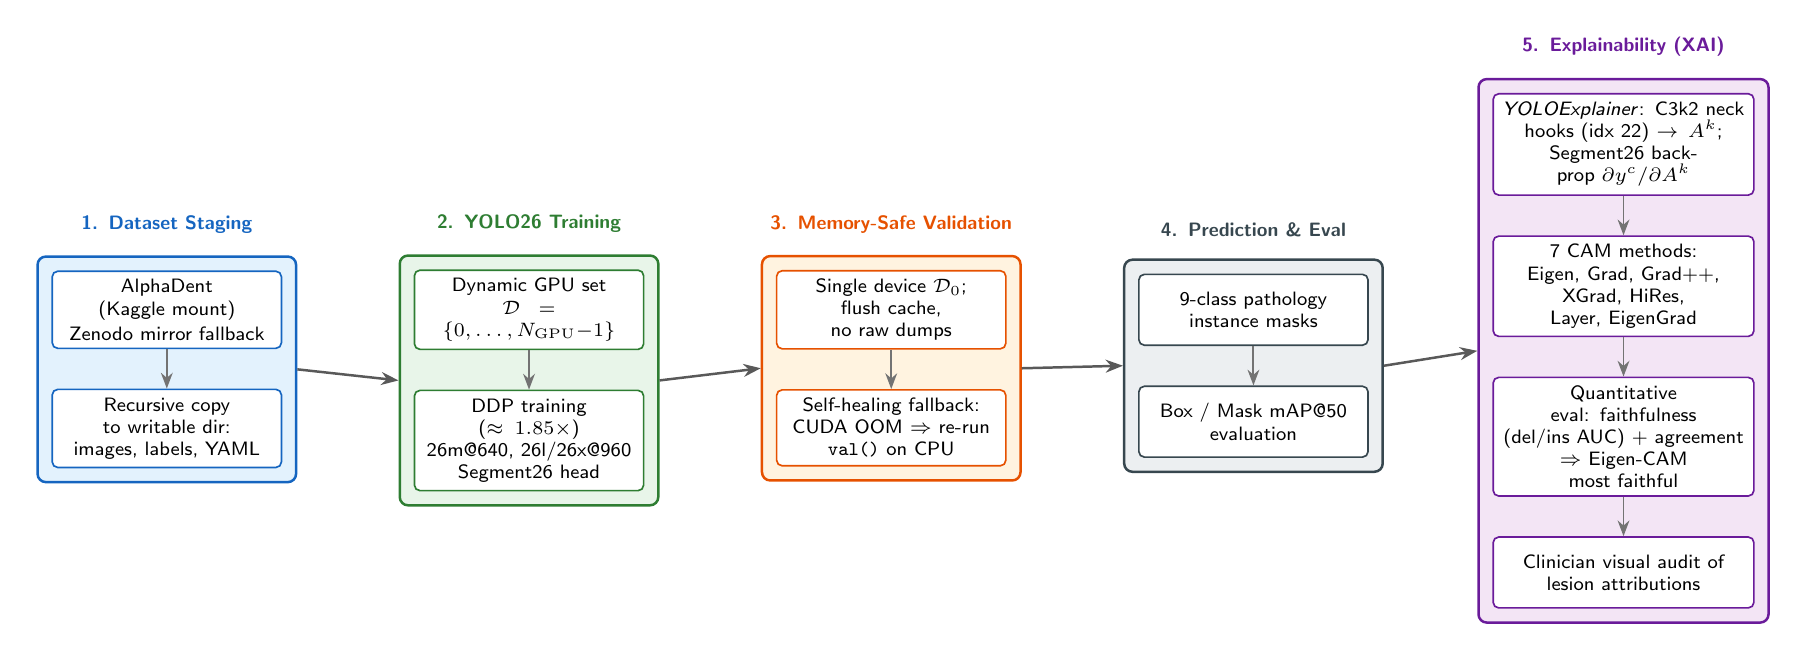
\begin{tikzpicture}[
  font=\scriptsize,
  box/.style={draw, rounded corners=2pt, align=center, inner sep=3pt,
              text width=27mm, minimum height=9mm, line width=0.6pt, fill=white},
  boxw/.style={box, text width=31mm},
  grp/.style={draw, rounded corners=3pt, inner sep=5pt, line width=0.9pt},
  ttl/.style={font=\bfseries\scriptsize, align=center, text width=33mm},
  arr/.style={-{Stealth[length=2.2mm]}, line width=0.9pt, draw=black!65},
  varr/.style={-{Stealth[length=2.0mm]}, line width=0.7pt, draw=black!55}
]
\def\yc{-21mm}   % vertical-center shift for the 2-box stages

% STAGE 1
\node[box, draw=cDataB] (a1) at (0mm,\yc) {AlphaDent (\mbox{Kaggle} mount)\\[1pt] Zenodo mirror fallback};
\node[box, draw=cDataB, below=5mm of a1] (a2) {Recursive copy to writable dir:\\ images, labels, YAML};
\draw[varr] (a1) -- (a2);
\begin{scope}[on background layer]
\node[grp, draw=cDataB, fill=cData, fit=(a1)(a2)] (g1) {};
\end{scope}
\node[ttl, text=cDataB, above=1.5mm of g1.north] {1. Dataset Staging};

% STAGE 2
\node[box, draw=cTrainB] (b1) at (46mm,\yc) {Dynamic GPU set\\ $\mathcal{D}=\{0,\dots,N_{\mathrm{GPU}}{-}1\}$};
\node[box, draw=cTrainB, below=5mm of b1] (b2) {DDP training ($\approx\!1.85\times$)\\ 26m@640, 26l/26x@960\\ Segment26 head};
\draw[varr] (b1) -- (b2);
\begin{scope}[on background layer]
\node[grp, draw=cTrainB, fill=cTrain, fit=(b1)(b2)] (g2) {};
\end{scope}
\node[ttl, text=cTrainB, above=1.5mm of g2.north] {2. YOLO26 Training};

% STAGE 3
\node[box, draw=cValB] (c1) at (92mm,\yc) {Single device $\mathcal{D}_0$;\\ flush cache, no raw dumps};
\node[box, draw=cValB, below=5mm of c1] (c2) {Self-healing fallback:\\ CUDA OOM $\Rightarrow$ re-run\\ \texttt{val()} on CPU};
\draw[varr] (c1) -- (c2);
\begin{scope}[on background layer]
\node[grp, draw=cValB, fill=cVal, fit=(c1)(c2)] (g3) {};
\end{scope}
\node[ttl, text=cValB, above=1.5mm of g3.north] {3. Memory-Safe Validation};

% STAGE 4
\node[box, draw=cOutB] (d1) at (138mm,\yc) {9-class pathology\\ instance masks};
\node[box, draw=cOutB, below=5mm of d1] (d2) {Box / Mask mAP@50\\ evaluation};
\draw[varr] (d1) -- (d2);
\begin{scope}[on background layer]
\node[grp, draw=cOutB, fill=cOut, fit=(d1)(d2)] (g4) {};
\end{scope}
\node[ttl, text=cOutB, above=1.5mm of g4.north] {4. Prediction \& Eval};

% STAGE 5 (tallest, anchored at top y=0)
\node[boxw, draw=cXAIB] (e1) at (185mm,0mm) {\textit{YOLOExplainer}: C3k2 neck hooks (idx 22) $\to A^k$;\\ Segment26 backprop $\partial y^c/\partial A^k$};
\node[boxw, draw=cXAIB, below=5mm of e1] (e2) {7 CAM methods: Eigen, Grad, Grad++,\\ XGrad, HiRes, Layer, EigenGrad};
\node[boxw, draw=cXAIB, below=5mm of e2] (e3) {Quantitative eval: faithfulness\\ (del/ins AUC) + agreement\\ $\Rightarrow$ Eigen-CAM most faithful};
\node[boxw, draw=cXAIB, below=5mm of e3] (e4) {Clinician visual audit of\\ lesion attributions};
\draw[varr] (e1) -- (e2);
\draw[varr] (e2) -- (e3);
\draw[varr] (e3) -- (e4);
\begin{scope}[on background layer]
\node[grp, draw=cXAIB, fill=cXAI, fit=(e1)(e2)(e3)(e4)] (g5) {};
\end{scope}
\node[ttl, text=cXAIB, above=1.5mm of g5.north] {5. Explainability (XAI)};

% INTER-STAGE ARROWS (aligned to common center line)
\draw[arr] (g1.east) -- (g2.west);
\draw[arr] (g2.east) -- (g3.west);
\draw[arr] (g3.east) -- (g4.west);
\draw[arr] (g4.east) -- (g5.west);

\end{tikzpicture}
\end{document}
